\documentclass[11pt]{amsart}
\usepackage{geometry}                % See geometry.pdf to learn the layout options. There are lots.
\geometry{letterpaper}                   % ... or a4paper or a5paper or ... 
%\geometry{landscape}                % Activate for for rotated page geometry
%\usepackage[parfill]{parskip}    % Activate to begin paragraphs with an empty line rather than an indent
\usepackage{graphicx}
\usepackage{subfigure}
\usepackage{enumitem}
\usepackage{amssymb}
\usepackage{epstopdf}
\DeclareGraphicsRule{.tif}{png}{.png}{`convert #1 `dirname #1`/`basename #1 .tif`.png}

\title{Unordered Selections Activity}
\author{Math 300}
%\date{}                                           % Activate to display a given date or no date

\begin{document}
\maketitle
%\section{x}
%\subsection{}


{\bf Example of a big general discrete math problem}:  An {\bf down-right path} on a $n \times n$ grid is a sequence $2n$ steps going either down or right at each step starting at the upper-left corner and ending and the bottom-right corner. Two examples of a $3 \times 3$ grid is pictured below.   How many different down-right paths are there on a $n \times n$ grid?

\begin{figure}[h]
  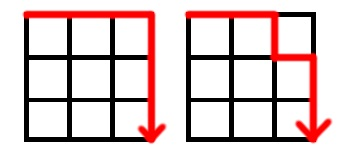
\includegraphics[scale=.60]{paths}
%  
\includegraphics[scale=.60]{path2}
   \caption{Two down-right paths on a $3 \times 3$ grid.}
\end{figure}

When facing a general problem like this, it's always a good idea to figure out what is going on for small $n$.  That is $n=1$, $n=2$, $n=3$ and so on.  \underline{Draw pictures of the $n=1$ and $n=2$ cases}.  
\vfill

Since there are six different solutions for $n=2$,  we might not want to continue to $n=3$ with this process be cause there may be so many that it's hard to figure out repeated drawings.


\pagebreak

Now that we have a good idea of the objects we are dealing with, it may be worth creating an easier model to work with, rather than drawing a bunch of picture.  An important observation here is that every picture can be turned into a list of directions R for right and D for down.  In this way the information in the above picture can be recored as RRRDDD and RRDRDD.  That is we need a string consisting of 3 Rs and 3 Ds. Can we create a stage based process to create such strings?\\


Consider the two stage process to create a length 6 string with 3 Rs and 3 Ds.\\

\begin{enumerate}[noitemsep, topsep=0pt, parsep=0pt, partopsep=0pt]
\item From the 6 locations choose 3 of them to place Rs.
\item From the remaining 3 locations choose 3 of them to place Ds.\\
\end{enumerate}


\underline{Questions:}
\begin{enumerate}[noitemsep, topsep=0pt, parsep=0pt, partopsep=0pt]
\item In the first stage are we allowed to repeat choices of location?
\item In the first stage does the order of choosing locations matter?  How can you check?
\item How many ways are there to do stage 1?
\item In the second stage why are we only choosing 3 locations?
\item In the second stage are we allowed to repeat choices of location?
\item In the second stage does the order of choosing locations matter?
\item How many ways are there to do stage 2?\\
\end{enumerate}
\vfill
Now consider strings of length 6 made with the following characters R,R,R,D,d, $\delta$.  Modify the above stage-based process to figure out how many strings can be created with those 6 characters.  Finally can you answer the general question:  How many different down-right paths are there on a $n \times n$ grid?


\end{document}  